\documentclass[a4paper,10pt]{article}
\usepackage[utf8]{inputenc}
\usepackage{amsmath}
\usepackage{subcaption}
\usepackage{notoccite}
\usepackage{xargs}                      % Use more than one optional parameter in a new commands
\usepackage[pdftex,dvipsnames]{xcolor}  % Coloured text etc.
\usepackage[colorinlistoftodos,prependcaption,textsize=tiny]{todonotes}
% note: disable any of the following commands by adding 'disable' as a first option after \todo
% see example with the third one
\newcommandx{\tobecompleted}[2][1=]{\todo[linecolor=red,backgroundcolor=red!25,
bordercolor=red,#1]{#2}}
\newcommandx{\thiswillnotshow}[2][1=]{\todo[disable,linecolor=OliveGreen,
backgroundcolor=OliveGreen!25,bordercolor=OliveGreen,#1]{#2}}

\DeclareMathOperator*{\argmin}{argmin} 
\DeclareMathOperator*{\argmax}{argmax} 

%opening
\title{PRIM Project\\ Segmentation of skin lesions}
\author{Roman Fenioux}

\begin{document}
\maketitle
\newpage
\begin{abstract}
In this project I will compare different segmentation methods for skin lesions. 
\tobecompleted{intro about skin lesion, importance, etc...}
\end{abstract}

\section{Segmentation}
\subsection{Thresholding}
\paragraph{}
The easiest method that comes to mind is thresholding since the skin lesions are 
usually darker than the surrounding skin. Given a grayscale image, we can 
classify pixels as being part of the region of interest (ROI) or of the 
background based on their intensities.
\paragraph{} Otsu~\cite{Otsu1979} \tobecompleted{Otsu algorithm description}
Our objective is to find a good threshold to separate the lesion from the 
surrounding skin. Otsu's approach consist seeing the histogram as a probability 
distribution, and then choosing the threshold that maximizes the separability 
measure $\eta$ or equivalently the variance $\sigma_B^2$ between the two classes 
obtained, as defined in equation \ref{eq:otsuvariance}.

\begin{equation} \label{eq:otsuvariance}
  \sigma_B^2 = \omega_0 (\mu_0 - \mu_T)^2 + \omega_1 (\mu_1 - \mu_T)^2 
\end{equation}
\begin{equation} \label{eq:optimthresh}
  k^* = \argmax_{1<k<L} \sigma_B^2(k)   
\end{equation}

\subsection{Region based segmentation}
\paragraph{} Statistical Region Merging~\cite{nock_statistical_2004} has been 
used by Celebi and al~\cite{celebi_border_2008} to perform a fast and efficient 
segmentation of skin lesions. This approach consists in merging regions in a particular order, with a statistical criterion.


\section{Pre-processing}
\subsection{Hair removal}
\paragraph{} Dullrazor~\cite{Dullrazor1997} algorithm is a standard method for 
hair removal. It consists in the following steps:
\begin{enumerate}
 \item Locating dark hair with a grayscale morphological closing operation with 
vertical, horizontal and diagonals structure elements on the three RGB channels. 
We obtain the hair mask by thresholding the absolute difference with the 
original image.
 \item Denoising the hair mask and interpolating the hair pixels with neighbor 
non-hair pixels. 
 \item Removing the remaining hair artefacts with an adapted median filter, only 
applied on the pixels located in the enlarged hair regions
 (morphological dilatation of the hair mask).
\end{enumerate}


\subsection{Color space}
The segmentation performance is influence by the colorspace used. Some methods 
\tobecompleted{cite them} simply use the blue channel from RGB colorspace, but 
Garnavi, Celebi and al~\cite{Garnavi2010} have shown that, at least for a 
threshold-based approach, the X channel from CIE-XYZ color space gives better 
performances.

\begin{figure}

  \begin{subfigure}{0.7\textwidth}
    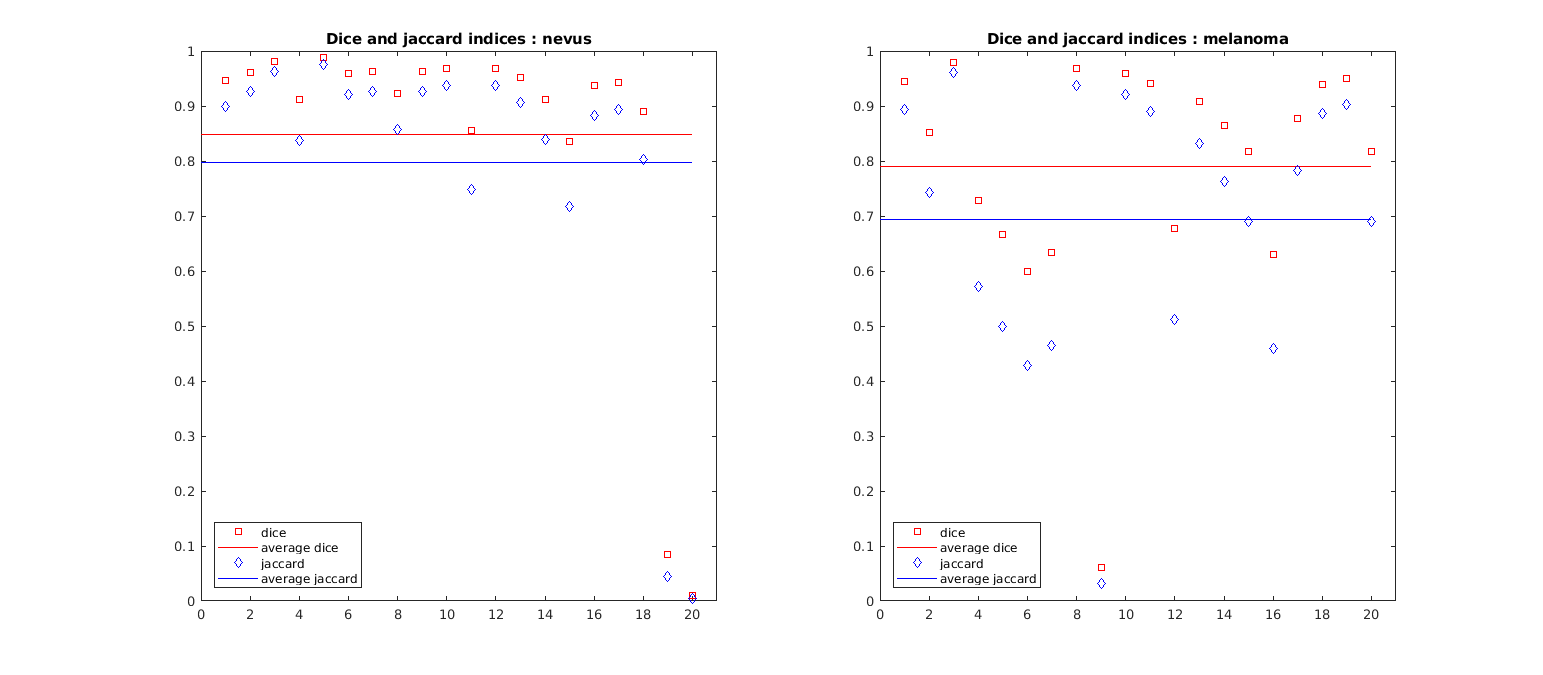
\includegraphics[width=0.9\linewidth]{../results/color-channel-influence/base-evaluation/otsu-dice-jaccard-B.png} 
    \caption{blue channel}
    \label{fig:otsu-blue}
  \end{subfigure}
  \begin{subfigure}{0.7\textwidth}
    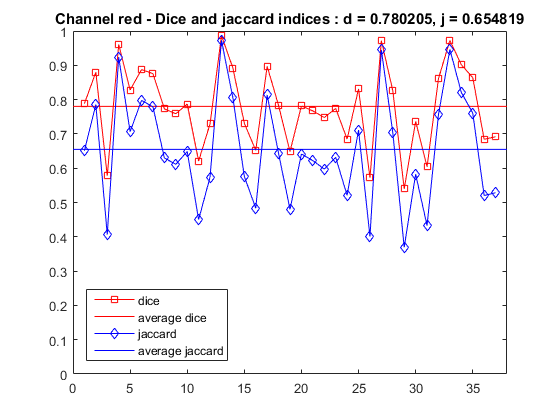
\includegraphics[width=0.9\linewidth]{../results/color-channel-influence/base-evaluation/otsu-dice-jaccard-R.png}
    \caption{red channel}
    \label{fig:otsu-red}
  \end{subfigure}
  \begin{subfigure}{0.7\textwidth}
    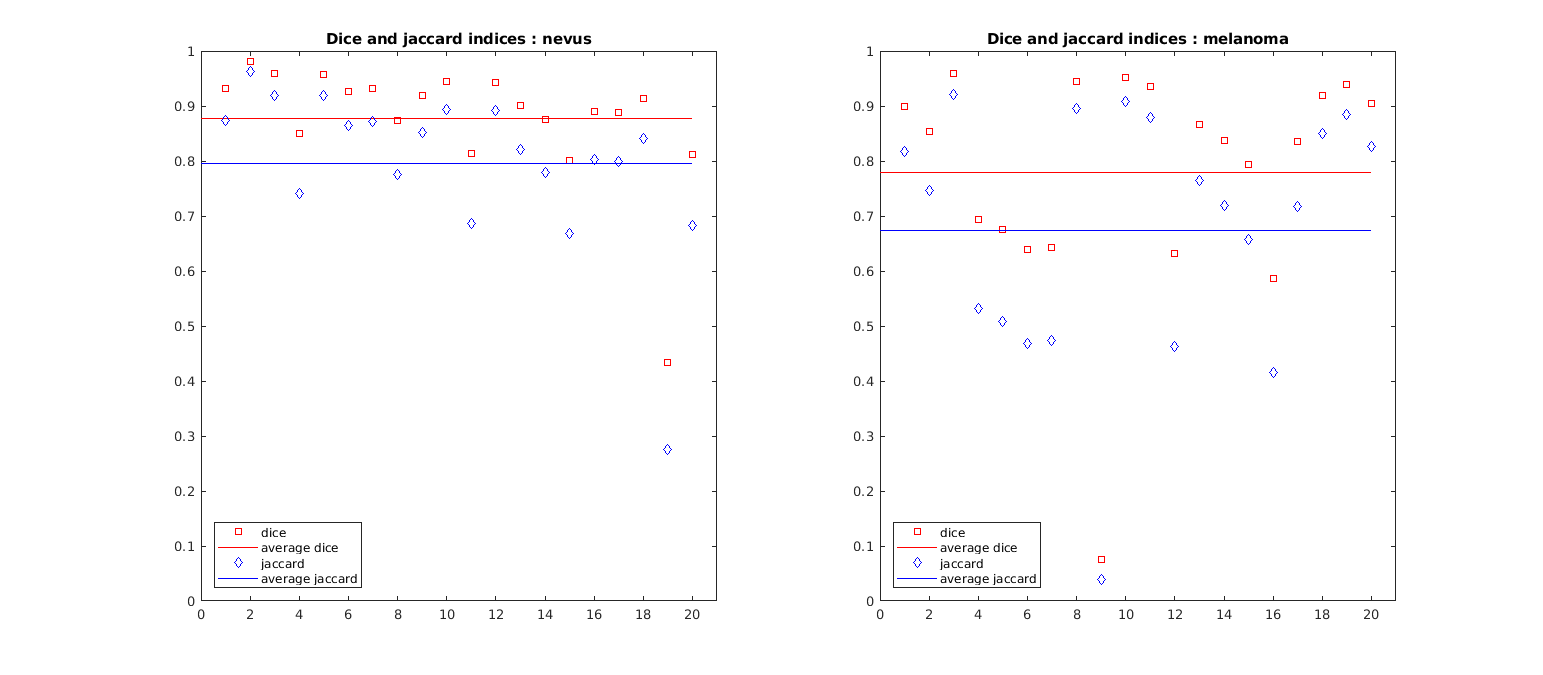
\includegraphics[width=0.9\linewidth]{../results/color-channel-influence/base-evaluation/otsu-dice-jaccard-G.png}
    \caption{green channel}
    \label{fig:otsu-green}
  \end{subfigure}
  \begin{subfigure}{0.7\textwidth}
    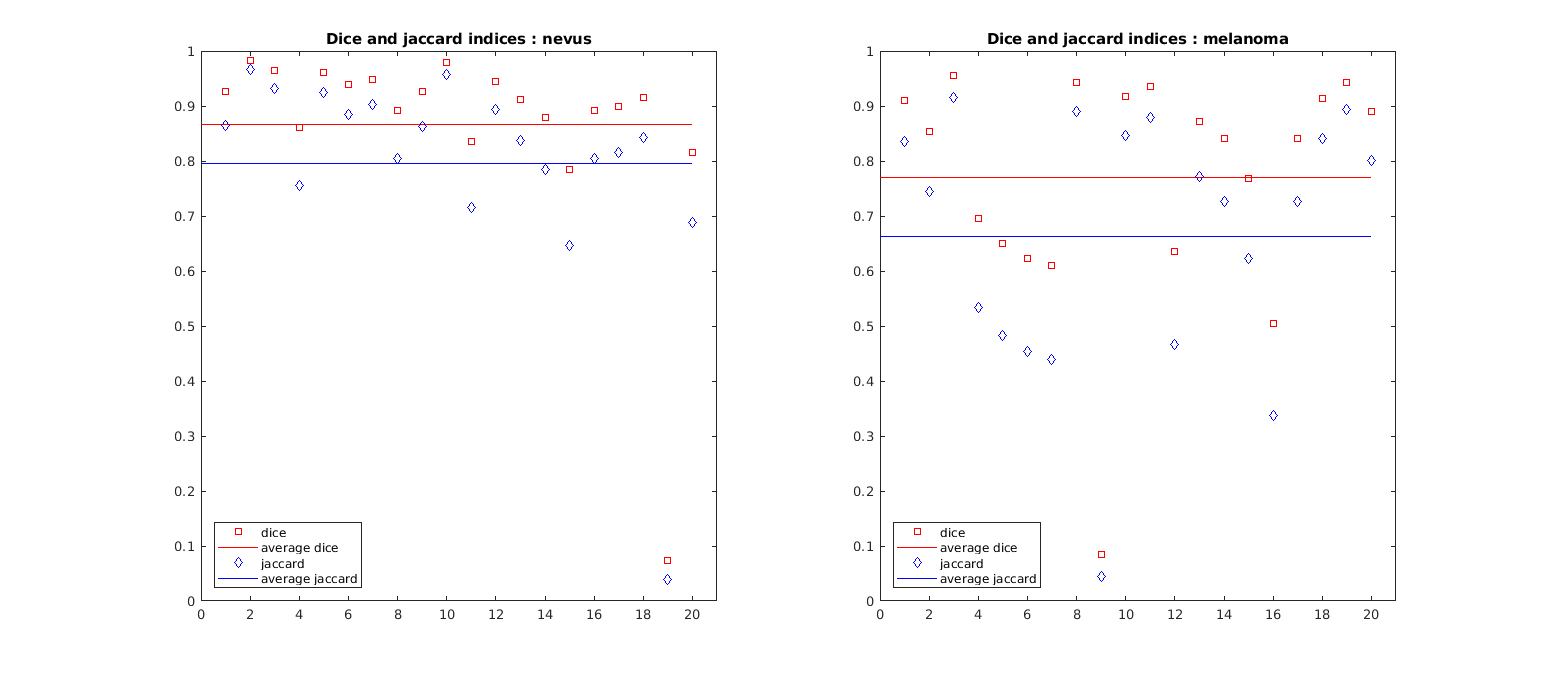
\includegraphics[width=0.9\linewidth]{../results/color-channel-influence/base-evaluation/otsu-dice-jaccard-meanRGB.png}
    \caption{RGB average}
    \label{fig:otsu-mean}
  \end{subfigure}
  \begin{subfigure}{0.7\textwidth}
    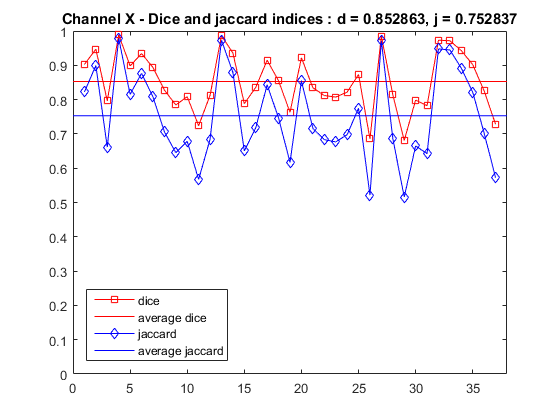
\includegraphics[width=0.9\linewidth]{../results/color-channel-influence/base-evaluation/otsu-dice-jaccard-X.png}
    \caption{channel X from CIE-XYZ}
    \label{fig:otsu-X}
  \end{subfigure}

  \caption{Color channel influence on Otsu thresholding performances}
  \label{fig:color-channel-otsu}
\end{figure} \tobecompleted{unclear ! not the best way to show these results... }


\bibliographystyle{plain}
\bibliography{PRIM-rapport}

\end{document}
